\documentclass{article}
\usepackage[utf8]{inputenc}
\usepackage{graphicx}
\usepackage{fancyvrb}
\graphicspath{{./images}}

\title{COS30031 Games Programming\\Research Project Report}
\author{Daniel Coady 102084174}
\date{18/10/2021}

\begin{document}

\maketitle

\pagebreak

\tableofcontents

\pagebreak

% TODO: come back to this once we have a conclusion written
\begin{abstract}
    Put the abstract here once we actually have one!
\end{abstract}

\section{Introduction}
\subsection{Background}
Game architecture is an art, one that is truly hard to learn and master. In
fact, there are many experts and experienced developers who disagree frequently
on the topic of how the backbone of games should be structured. This happens for
a variety of reasons, but more often than not we will see two aspects of various
architectures compared: the usability or maintainability, and the performance.

When we talk about the usability or maintainability of something, we refer to
how easy it is to work with. Of interest to us is the ergonomics related to
developing with and extending on a given architecture as the needs of a solution
expands in scope. Performance on the other hand is far more straightforward--how
fast is it? Both aspects are incredibly important when weighing up which
architecture is most appropriate to you, your project, and your needs.

\subsection{Purpose of This Research}
Using the metrics outlined earlier, I aim to compare and contrast four different
architectures. This will involve deep dives into every architecture, dissecting
how all of them work and what their purposes are. My hope is that through this
research presented in this report, the reader may be able to:

\begin{itemize}
    \item Understand what each architecture is, and how they work
    \item Understand the purpose of each architecture
    \item Understand the use case for each architecture
    \item Come to their own conclusions regarding choices in game architecture
\end{itemize}

\section{Methodology}
In order to test the various aspects of each of these architectures, I have had
to formulate a series of tests and establish a common testing environment for
each of these tests to be run within.

\subsection{Tests}
All tests will be done with a simple set of entities. These entities will be
represented by squares in a graphical window, and they will move with a fixed
velocity. When an entity reaches the edge of the window, it will then loop back
around to the other side of the window. To add an extra layer of complexity to
the processing of the entities, a random amount of entities will also colour
shift while moving. Data will be tracked in the form of average cycles per
second and the output provided by valgrind's cachegrind tool.

To ensure we collect as much useful data as possible, I will extend this basis
for testing in three key ways:

\subsubsection{Static}
The test will be run with 250,000 entities in the simulation over the course of
one minute. The purpose of this test is to understand at a high level how
compiler optimisation level affects the speed of each architecture.

\subsubsection{Ramp-up}
There will be multiple tests run for each architecture, starting at 100,000
entities and adding 100,000 with each subsequent test until 500,000 entities is
reached. Each test will be run over the course of one minute. The purpose of
this test is to understand at a high level how a given architecture scales up
given n amount of entities.

\subsubsection{Dynamic Ramp-up}
A single test will be run for each architecture that starts with 0 entities. For
each cycle performed, an entity will be added to the architecture until a limit
of 100,000 entities is hit. Once this limit has been hit, entities will start
being removed from the architecture until there are none left, and the time
taken to execute will be measured. The purpose of this test is to understand at
a high level how the overhead introduced by the creation and removal of entities
from an architecture affect the execution time of an application.

\subsection{Environment}
In order to test each of these architectures, a common environment for them to
run in has been established. This will take form of a simple front-end
abstraction I have written on top of the OpenGL 4.3 Core API, using GLFW for
windowing and other miscellaneous functionality. All code used for the
environment and development of tests will be written in C++, targeting the C++17
standard at a maximum. Something to note here is that I have elected to use
OpenGL 4.3 Core. This is because it is the first version of the OpenGL
specification to add compute shaders to the core profile, which will become
important later on for one of our architectures.

\section{Introduction to Tested Architectures}
This research has chosen to focus on four key architectures. The rationale
behind this is while it might not be exhaustive, it will provide meaningful
data points to inform how different styles and implementations of architecture
can affects the usability/maintainability and performance of your game. All
code mentioned will be available on
GitHub\footnote{https://github.com/pondodev/research-project} under the
Unlicense License.

\subsection{Architecture A--Pure Object Oriented}
Taking a more traditional and plain object oriented approach, we see what you
might expect from a more standard application's codebase. Since it is very pure
as far as object oriented architecture goes, much of the same goals of the
paradigm carry over to this architecture--that is, we want to maximise code
cohesion, minimise code coupling, and reduce overall code duplication. Most of
this is to ensure that at a high level, the codebase is as maintainable as
possible. There are a few notable parts that make up this architecture:

\begin{itemize}
    \item Engine
    \item[] The brains of the operation. Manages entities and their associated
            memory.

    \item Entity
    \item[] A base class for all entities in the architecture to inherit from.

    \item Colour Shift Entity
    \item[] A class which derives from the entity base class to add colour
            shifting functionality. 
\end{itemize}

\begin{figure}
\centering
\begin{BVerbatim}
class Entity {
public:
    Entity(
        unsigned int _id,
        glm::vec2 _position,
        glm::vec2 _velocity,
        glm::vec3 _color );
    virtual void update();
    unsigned int get_id();
    glm::vec2 get_position();
    glm::vec3 get_color();

protected:
    glm::vec3 color;

private:
    unsigned int id;
    glm::vec2 position;
    glm::vec2 velocity;
};
\end{BVerbatim}
\caption{Architecture A Entity class declaration}
\label{arch_a_entity_header}
\end{figure}

\begin{figure}
\centering
\begin{BVerbatim}
class ColorShiftEntity : public Entity {
public:
    ColorShiftEntity(
        unsigned int _id,
        glm::vec2 _position,
        glm::vec2 _velocity,
        glm::vec3 _color,
        glm::vec3 _color_velocity );
    void update() override;

private:
    glm::vec3 color_velocity;
};
\end{BVerbatim}
\caption{Architecture A ColorShiftEntity class declaration}
\label{arch_a_color_shift_entity_header}
\end{figure}

\begin{figure}
\centering
\begin{BVerbatim}
class Engine {
public:
    ~Engine();
    unsigned int add_entity(
        glm::vec2 _position,
        glm::vec2 _velocity,
        glm::vec3 _color );
    unsigned int add_entity(
        glm::vec2 _position,
        glm::vec2 _velocity,
        glm::vec3 _color,
        glm::vec3 _color_velocity );
    void remove_entity( unsigned int id );
    void pop_entity();
    std::vector<Entity*> get_entities();
    void update();

private:
    unsigned int current_entity_id = 0;
    std::vector<Entity*> entities;
};
\end{BVerbatim}
\caption{Architecture A Engine class declaration}
\label{arch_a_engine_header}
\end{figure}

Starting with the Entity class in figure \ref{arch_a_entity_header}, it contains
some basic information required to render a given entity to the provided render
target--a 2D position, a 2D velocity, and a colour with RGB components. We also
have some simple getter methods for acquiring the private and protected members
of the class, and an update method which simply will move the entity's position
by the given velocity vector.

The ColorShiftEntity class in figure \ref{arch_a_color_shift_entity_header} then
inherits from the Entity class and adds a new member to store colour velocity.
This colour velocity is also an RGB value which dictates how the colour of an
entity should shift with every update. It's for this reason that we have an
override for the update method, which will perform the same update functionality
as the base Entity class but will also apply the colour velocity.

Finally, the Engine class in figure \ref{arch_a_engine_header} which uses a
factory-like pattern. The engine is what a programmer would primarily be
interfacing with in order to operate the architecture. This is because it is
where one would create, manage, and update entities. It provides a method with
two overrides to create an entity--one override for regular entities and one
override for colour shifting entities. There is also a method to update every
single entity managed by the engine.

\subsection{Architecture B--Object Oriented Component Pattern}
This is an architecture many might be familiar with from general purpose engines
such as Unity or Unreal Engine 4. The core idea at play is that pure object
oriented approaches to game architecture aren't particularly conducive to how
games are generally programmed. In particular, there is the idea of an entity
having a series of "traits" which apply to it which in a purely object oriented
architecture would normally be implemented through means of inheritance.
However, this can be prone to many different types of issues such as deep,
complicated inheritance trees or ambiguity introduced through diamond
inheritance. To add to this, it becomes significantly less feasible to implement
this kind of architecture with a language such as C\# which does not allow for
multiple inheritance and would instead require you to use interfaces.

This is the core rationale behind the component pattern in object oriented
game architecture design--reduce the amount of inheritance required by storing
a collection of components which define traits of an entity, inside of an
entity. This also means that in languages like C\# which do not support
multiple inheritance, we can still implement this pattern in a clean and
maintainable manner. My implementation has 4 key parts:

\begin{itemize}
    \item Engine
    \item[] Much like the pure object oriented architecture, manages the
            creation, removal, and updating of entities.

    \item Entity
    \item[] A very bare bones class that has an id and collection of components.

    \item Component Base
    \item[] The base class from which all components that can define traits or
            behaviour of an entity will inherit from.

    \item Components
    \item[] Child classes of the component base class that will define specific
            traits or behaviour for entities it is applied to.
\end{itemize}

\begin{figure}
\centering
\begin{BVerbatim}
class Entity {
public:
    Entity();
    ~Entity();
    unsigned int get_id();
    void add_component( Component* c );
    void remove_component( unsigned int id );
    template <typename T>
    std::optional<T*> get_component() {
        std::optional<T*> to_return;

        for ( auto c : components ) {
            if ( typeid(*c) == typeid(T) ) {
                to_return = (T*)c;
                break;
            }
        }

        return to_return;
    }

private:
    static inline unsigned int next_id;
    unsigned int id;
    std::vector<Component*> components;
};
\end{BVerbatim}
\caption{Architecture B Entity class declaration}
\label{arch_b_entity_header}
\end{figure}

\begin{figure}
\centering
\begin{BVerbatim}
class Component {
public:
    Component();
    virtual unsigned int get_id(); // virtual so RTTI works

private:
    static inline unsigned int next_id;
    unsigned int id;
};
\end{BVerbatim}
\caption{Architecture B ComponentBase class declaration}
\label{arch_b_component_base_header}
\end{figure}

\begin{figure}
\centering
\begin{BVerbatim}
class MovementComponent : public Component {
public:
    MovementComponent( glm::vec2 _pos, glm::vec2 _vel );
    void move();
    glm::vec2 pos;

private:
    glm::vec2 vel;
};

class ColorComponent : public Component {
public:
    ColorComponent( glm::vec3 _value );
    void apply_velocity( glm::vec3 vel );
    glm::vec3 value;
};

class ColorVelocityComponent : public Component {
public:
    ColorVelocityComponent( glm::vec3 _value );
    glm::vec3 value;
};
\end{BVerbatim}
\caption{Architecture B Component class declarations}
\label{arch_b_components_header}
\end{figure}

\begin{figure}
\centering
\begin{BVerbatim}
class Engine {
public:
    ~Engine();
    void add_entity( Entity* entity );
    void remove_entity( unsigned int id );
    void pop_entity();
    std::optional<Entity*> get_entity( unsigned int id );
    std::vector<Entity*> get_all_entities();
    void update();

private:
    std::vector<Entity*> entities;
};
\end{BVerbatim}
\caption{Architecture B Engine class declaration}
\label{arch_b_engine_header}
\end{figure}

The Entity class is incredibly simple for the most part: an id, a vector of
components belonging to this entity, and methods to add/remove components from
an entity. There is one rather complex thing, however, and that is the template
method for getting a component from an entity. This method uses run time type
information (RTTI for short) to get an arbitrary component of a given type from
the vector of components.

The ComponentBase class in figure \ref{arch_b_component_base_header}, as
previously mentioned, will be the base class that all components inherit from.
It's simple for the most part, only really providing one getter method for the
component's id. However one curiosity here is that the method to get the id is
virtual, but we never override it in any of the classes that derive from it.
This is due to a quirk of C++ and it's design since type information isn't
available during run time in the same way we might expect it to be in something
like C\# and it's reflection feature. To get around this, there is RTTI which
can give us partial information on types during runtime, but it requires us to
do two things: provide a pointer, and implement at least one virtual method on
the base class to be inherited from.

Components as seen in figure \ref{arch_b_components_header} all inherit from the
ComponentBase class. This allows us to polymorphically store them in a
collection (which is exactly what we do in the Entity class) while still
providing unique functionality per component.

Finally there is the Engine class in figure \ref{arch_b_engine_header}. Much
like the pure object oriented architecture, the engine will manage all entities
and their associated memory appropriately. However, a key difference is that
creation of the entity is now an external responsibility to the engine and a
programmer would then need to register the created entity with the engine. This
is something I would classify as a design flaw in the implementation which, if
used in the real world, should be remedied. However for the purposes of these
tests it will be more than adequate to collect the necessary data.

\subsection{Architecture C--Entity Component System}
While by no means a new approach to game architecture with uses of it dating
back to 2001-2003\footnote{http://t-machine.org/index.php/2007/09/03/entity-systems-are-the-future-of-mmog-development-part-1/},
it is only in recent times where we have seen it truly come into it's own.
Entity component systems, often shortened down to ECS, are a performance first
architecture design which foregoes object oriented design in favour of data
oriented design. The key difference between the two paradigms is that while
object oriented design prioritises concepts such as ownership through means of
abstraction and encapsulation, data oriented design chooses to separate data
entirely from it's functionality. This is done through the 3 parts of an ECS
implementation:

\begin{itemize}
    \item Entities
    \item[] Abstract identifiers that are used to denote ownership over a
            registered component in the architecture.

    \item Components
    \item[] Simple, tightly packed data packets that can be considered a "state"
            belonging to an entity.

    \item Systems
    \item[] Functionality which operates over a collection of entities and it's
            select components that are registered to a given system, applying
            logic and functionality to the components.
\end{itemize}

\begin{figure}
\centering
\begin{BVerbatim}
typedef uint32_t Entity;
typedef enum {
    Movable       = 0b100,
    Color         = 0b010,
    ColorVelocity = 0b001
} ComponentFlag;
\end{BVerbatim}
\caption{Architecture C typedefs}
\label{arch_c_typedefs}
\end{figure}

\begin{figure}
\centering
\begin{BVerbatim}
struct MovableComponent {
    float pos_x;
    float pos_y;
    float vel_x;
    float vel_y;
};

struct ColorComponent {
    float r;
    float g;
    float b;
};

struct ColorVelocityComponent {
    float r;
    float g;
    float b;
};
\end{BVerbatim}
\caption{Architecture C component struct declarations}
\label{arch_c_components_header}
\end{figure}

\begin{figure}
\centering
\begin{BVerbatim}
class Engine {
public:
    Engine();
    ~Engine();
    std::optional<Entity> add_entity();
    void remove_entity( Entity id );
    int entity_has_component( Entity id, ComponentFlag component );

    void movement_system();
    void color_shift_system();

    MovableComponent* add_movable_component( Entity id );
    ColorComponent* add_color_component( Entity id );
    ColorVelocityComponent* add_color_velocity_component( Entity id );

    MovableComponent* get_movable_component( Entity id );
    ColorComponent* get_color_component( Entity id );
    ColorVelocityComponent* get_color_velocity_component( Entity id );

private:
    std::queue<Entity> available_entities;
    std::vector<Entity> movement_system_entities;
    std::vector<Entity> color_shift_system_entities;

    ComponentFlag* entity_component_flags;
    MovableComponent* movable_components;
    ColorComponent* color_components;
    ColorVelocityComponent* color_velocity_components;
};
\end{BVerbatim}
\caption{Architecture C Engine class declaration}
\label{arch_c_engine_header}
\end{figure}

The first thing of note are a couple of simple typedefs that have been created,
as seen in figure \ref{arch_c_typedefs}. The first is for entities, which
defines their id as an unsigned 32-bit integer. The second is an enum flag set
which we can bitwise-or together to indicate what components have been set on an
entity.

Components, as mentioned before, are incredibly simple. Figure
\ref{arch_c_components_header} shows that each component is nothing more than a
struct with primitive data within.

The Engine class in figure \ref{arch_c_engine_header} is actually somewhat of a
simplification of what you might expect in a more general purpose ECS
implementation. This is because normally there are separate manager classes for
each of the parts of an ECS, however for the purpose of this research I have
elected to simplify it down for demonstration purposes and simplicity.

Within this Engine class we have some methods for adding and removing entities,
functionality normally delegated to an entity manager. We also have parts of
what might be expected from a component manager in the form of methods to
add/get components for an entity and tightly packed arrays which contain the
components. The final piece of the puzzle then are the systems, which come in
two parts. First are the two system methods which perform the actual
functionality of a given system, and second are the vectors which contain all
the entity ids which are registered to be worked on by a given system.

As a final note, I'll mention that I owe a great deal to Austin Morlan as their
ECS implementation\footnote{https://austinmorlan.com/posts/entity\_component\_system/}
inspired much of my own.

\subsection{Architecture D--Entity Component System With\\Compute Shaders}
This is identical to Architecture A with one key difference: we use the GPU to
run the systems in the ECS implementation. In theory this should provide
incredible performance benefits to our architecture since GPUs are incredibly
fast at parallel floating point computations. However, much to my own 
disappointment, I was not able to implement it fully into an ECS implementation
for reasons that will be mentioned later. I have, however, successfully written
computer shaders in OpenGL\footnote{https://github.com/pondodev/opengl\_compute}
so will be able to comment more on other aspects of it. This does unfortunately
mean that I have been unable to collect any data on it and as such, will not be
able to report on the performance of it.

\clearpage

\section{Data}
The following sections display the data visualisations for each test run.

\subsection{Architecture A}
\begin{figure}[!h]
\centering
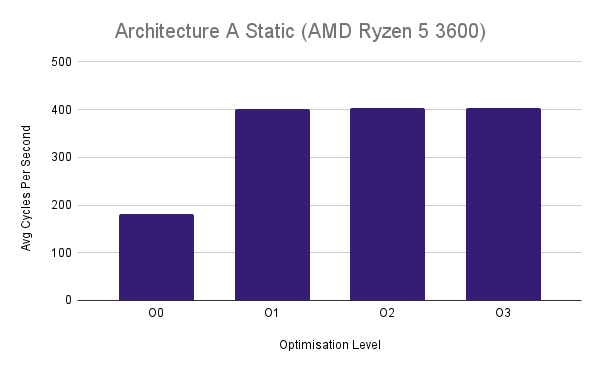
\includegraphics[scale=0.5]{Architecture A Static (AMD Ryzen 5 3600).png}
\label{arch_a_static_pc}
\caption{Architecture A Static Test (AMD Ryzen 5 3600)}
\end{figure}

\begin{figure}[!h]
\centering
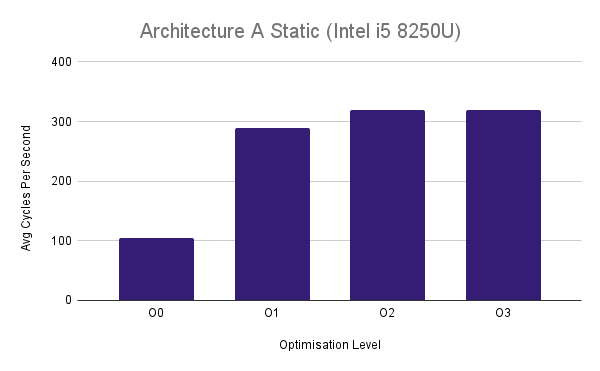
\includegraphics[scale=0.5]{Architecture A Static (Intel i5 8250U).png}
\label{arch_a_static_laptop}
\caption{Architecture A Static Test (Intel i5 8250U)}
\end{figure}

\begin{figure}[!h]
\centering
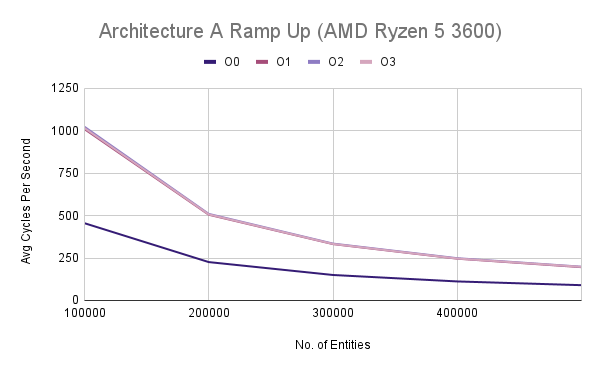
\includegraphics[scale=0.5]{Architecture A Ramp Up (AMD Ryzen 5 3600).png}
\label{arch_a_ramp_up_pc}
\caption{Architecture A Ramp Up Test (AMD Ryzen 5 3600)}
\end{figure}

\begin{figure}[!h]
\centering
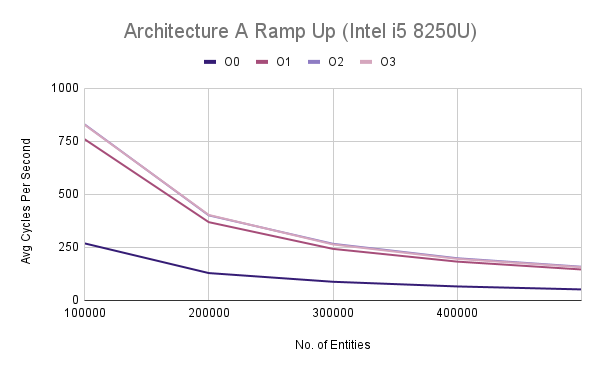
\includegraphics[scale=0.5]{Architecture A Ramp Up (Intel i5 8250U).png}
\label{arch_a_ramp_up_laptop}
\caption{Architecture A Ramp Up Test (Intel i5 8250U)}
\end{figure}

\begin{figure}[!h]
\centering
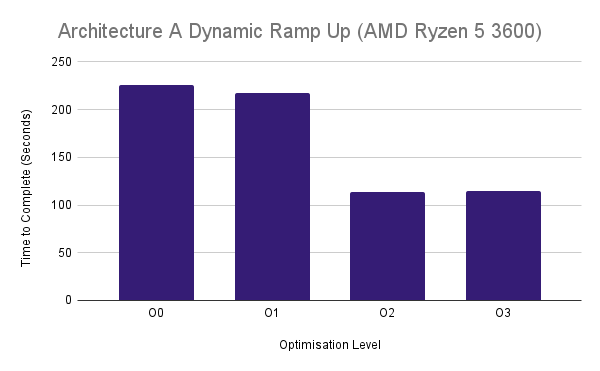
\includegraphics[scale=0.5]{Architecture A Dynamic Ramp Up (AMD Ryzen 5 3600).png}
\label{arch_a_dynamic_ramp_up_pc}
\caption{Architecture A Dynamic Ramp Up Test (AMD Ryzen 5 3600)}
\end{figure}

\begin{figure}[!h]
\centering
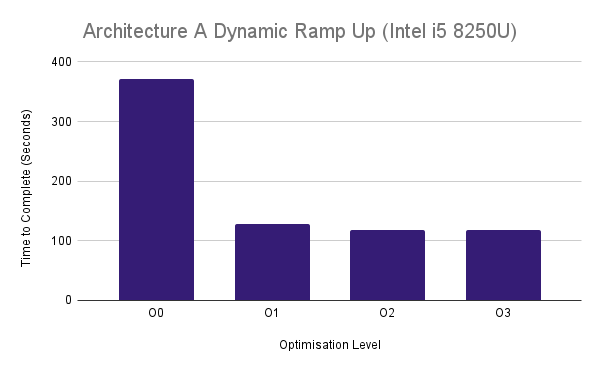
\includegraphics[scale=0.5]{Architecture A Dynamic Ramp Up (Intel i5 8250U).png}
\label{arch_a_dynamic_ramp_up_laptop}
\caption{Architecture A Dynamic Ramp Up Test (Intel i5 8250U)}
\end{figure}

\clearpage

\subsection{Architecture B}
\begin{figure}[!h]
\centering
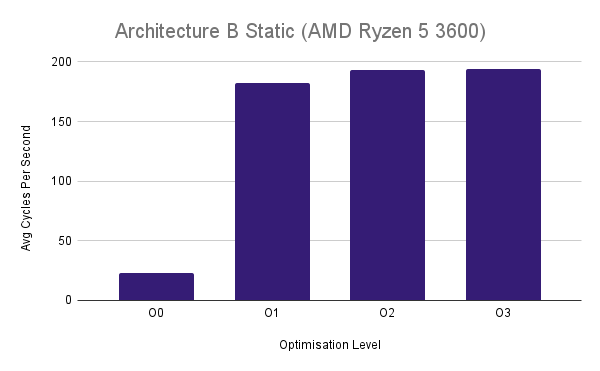
\includegraphics[scale=0.5]{Architecture B Static (AMD Ryzen 5 3600).png}
\label{arch_b_static_pc}
\caption{Architecture B Static Test (AMD Ryzen 5 3600)}
\end{figure}

\begin{figure}[!h]
\centering
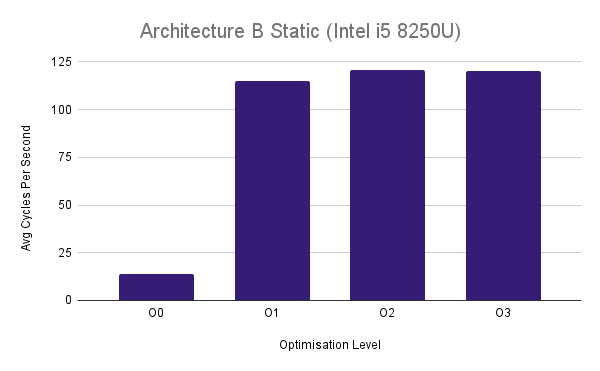
\includegraphics[scale=0.5]{Architecture B Static (Intel i5 8250U).png}
\label{arch_b_static_laptop}
\caption{Architecture B Static Test (Intel i5 8250U)}
\end{figure}

\begin{figure}[!h]
\centering
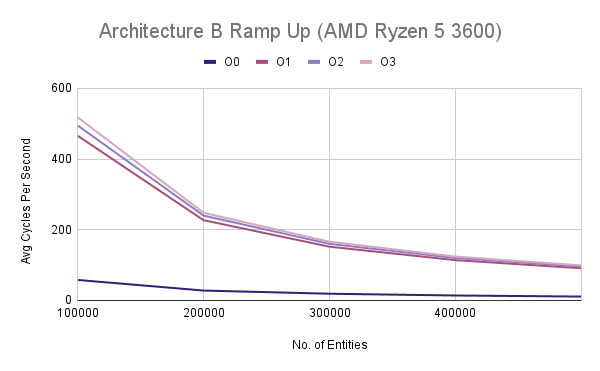
\includegraphics[scale=0.5]{Architecture B Ramp Up (AMD Ryzen 5 3600).png}
\label{arch_b_ramp_up_pc}
\caption{Architecture B Ramp Up Test (AMD Ryzen 5 3600)}
\end{figure}

\begin{figure}[!h]
\centering
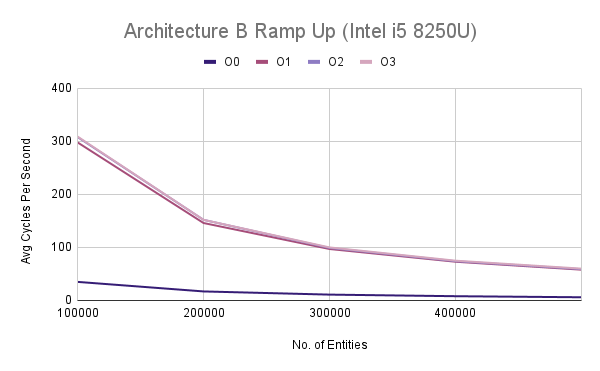
\includegraphics[scale=0.5]{Architecture B Ramp Up (Intel i5 8250U).png}
\label{arch_b_ramp_up_laptop}
\caption{Architecture B Ramp Up Test (Intel i5 8250U)}
\end{figure}

\begin{figure}[!h]
\centering
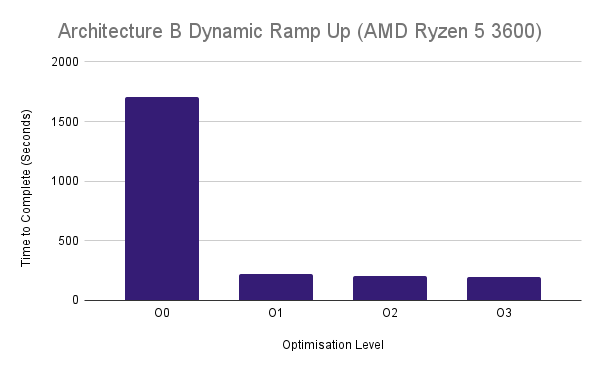
\includegraphics[scale=0.5]{Architecture B Dynamic Ramp Up (AMD Ryzen 5 3600).png}
\label{arch_b_dynamic_ramp_up_pc}
\caption{Architecture B Dynamic Ramp Up Test (AMD Ryzen 5 3600)}
\end{figure}

\begin{figure}[!h]
\centering
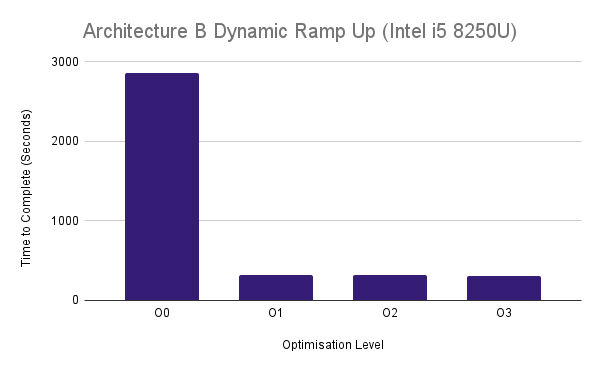
\includegraphics[scale=0.5]{Architecture B Dynamic Ramp Up (Intel i5 8250U).png}
\label{arch_b_dynamic_ramp_up_laptop}
\caption{Architecture B Dynamic Ramp Up Test (Intel i5 8250U)}
\end{figure}

\clearpage

\subsection{Architecture C}
\begin{figure}[!h]
\centering
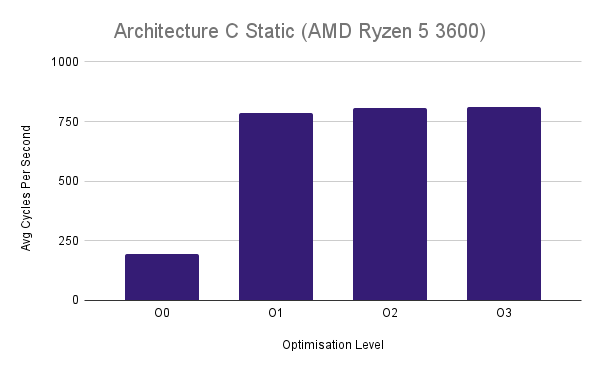
\includegraphics[scale=0.5]{Architecture C Static (AMD Ryzen 5 3600).png}
\label{arch_c_static_pc}
\caption{Architecture C Static Test (AMD Ryzen 5 3600)}
\end{figure}

\begin{figure}[!h]
\centering
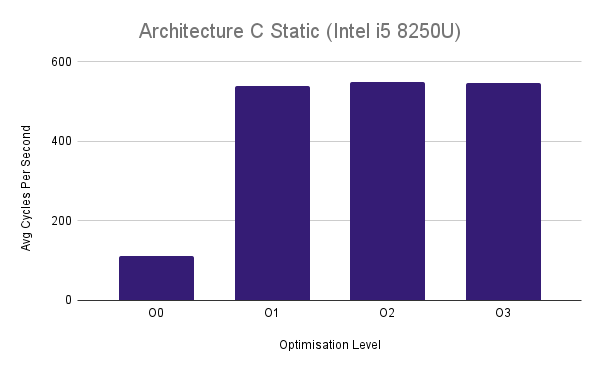
\includegraphics[scale=0.5]{Architecture C Static (Intel i5 8250U).png}
\label{arch_c_static_laptop}
\caption{Architecture C Static Test (Intel i5 8250U)}
\end{figure}

\begin{figure}[!h]
\centering
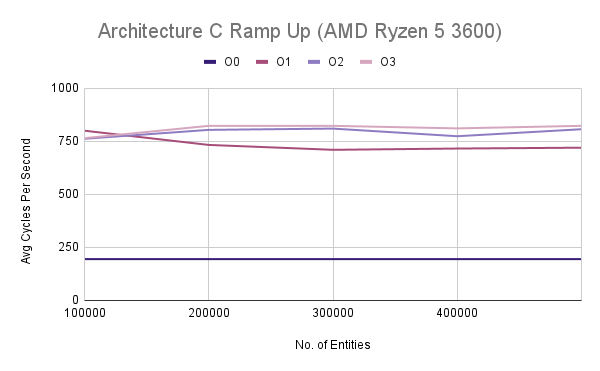
\includegraphics[scale=0.5]{Architecture C Ramp Up (AMD Ryzen 5 3600).png}
\label{arch_c_ramp_up_pc}
\caption{Architecture C Ramp Up Test (AMD Ryzen 5 3600)}
\end{figure}

\begin{figure}[!h]
\centering
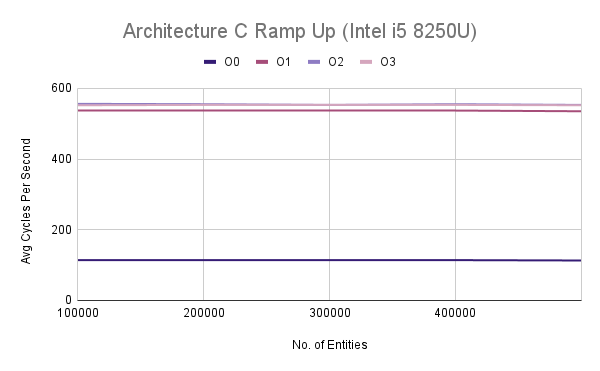
\includegraphics[scale=0.5]{Architecture C Ramp Up (Intel i5 8250U).png}
\label{arch_c_ramp_up_laptop}
\caption{Architecture C Ramp Up Test (Intel i5 8250U)}
\end{figure}

\begin{figure}[!h]
\centering
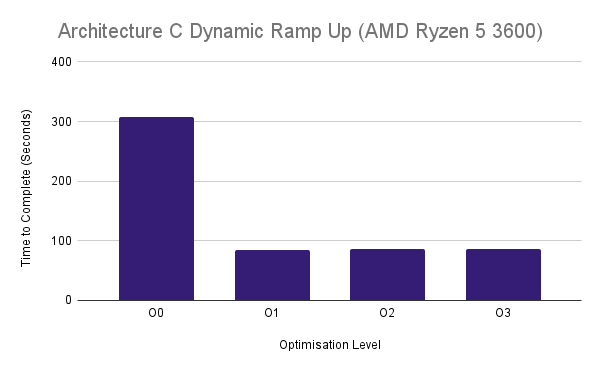
\includegraphics[scale=0.5]{Architecture C Dynamic Ramp Up (AMD Ryzen 5 3600).png}
\label{arch_c_dynamic_ramp_up_pc}
\caption{Architecture C Dynamic Ramp Up Test (AMD Ryzen 5 3600)}
\end{figure}

\begin{figure}[!h]
\centering
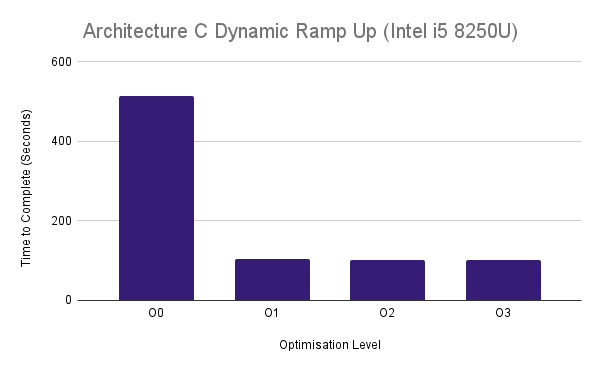
\includegraphics[scale=0.5]{Architecture C Dynamic Ramp Up (Intel i5 8250U).png}
\label{arch_c_dynamic_ramp_up_laptop}
\caption{Architecture C Dynamic Ramp Up Test (Intel i5 8250U)}
\end{figure}

\clearpage

\subsection{Architecture Comparisons}
\begin{figure}[!h]
\centering
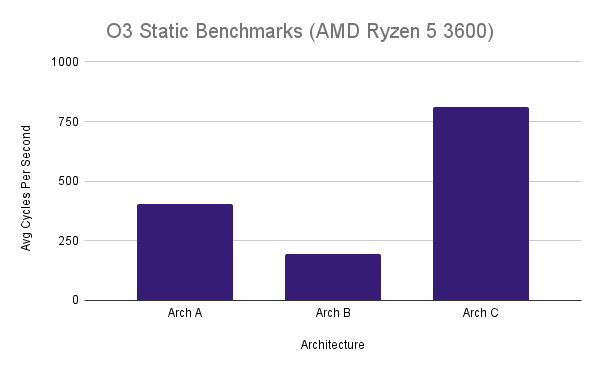
\includegraphics[scale=0.5]{O3 Static Benchmarks (AMD Ryzen 5 3600).png}
\label{pc_static_tests}
\caption{Static Tests (AMD Ryzen 5 3600)}
\end{figure}

\begin{figure}[!h]
\centering
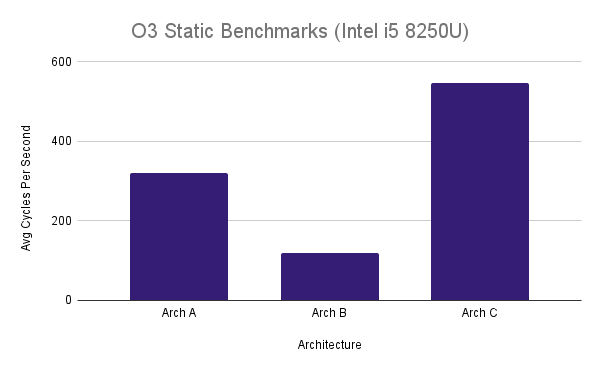
\includegraphics[scale=0.5]{O3 Static Benchmarks (Intel i5 8250U).png}
\label{lapotp_static_tests}
\caption{Static Tests (Intel i5 8250U)}
\end{figure}

\begin{figure}[!h]
\centering
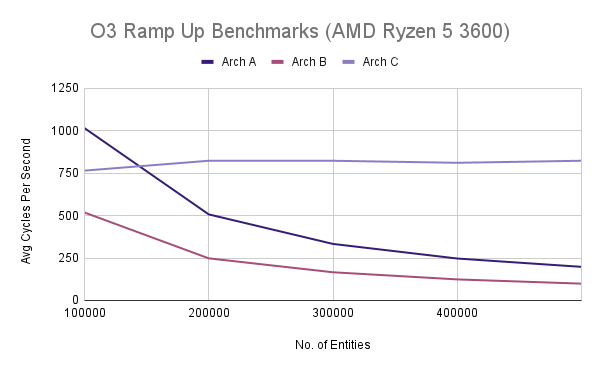
\includegraphics[scale=0.5]{O3 Ramp Up Benchmarks (AMD Ryzen 5 3600).png}
\label{pc_ramp_up_tests}
\caption{Ramp Up Tests (AMD Ryzen 5 3600)}
\end{figure}

\begin{figure}[!h]
\centering
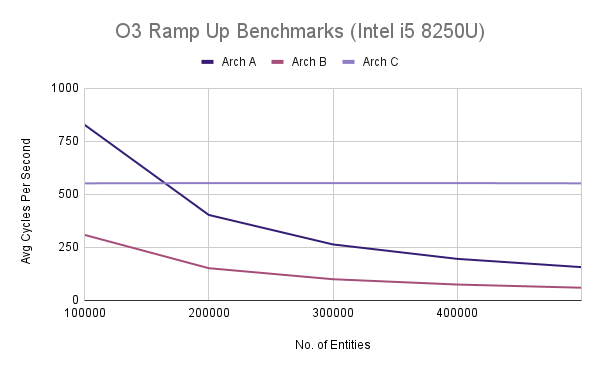
\includegraphics[scale=0.5]{O3 Ramp Up Benchmarks (Intel i5 8250U).png}
\label{lapotp_ramp_up_tests}
\caption{Ramp Up Tests (Intel i5 8250U)}
\end{figure}

\begin{figure}[!h]
\centering
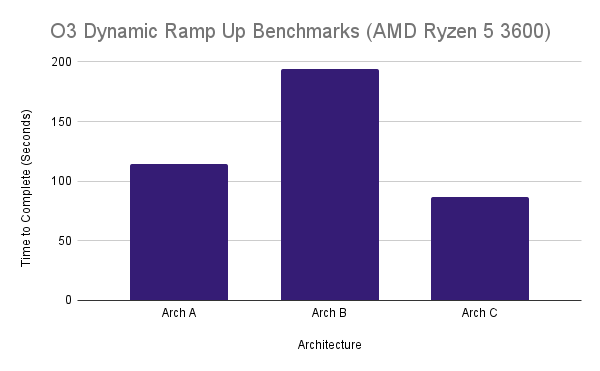
\includegraphics[scale=0.5]{O3 Dynamic Ramp Up Benchmarks (AMD Ryzen 5 3600).png}
\label{pc_dynamic_ramp_up_tests}
\caption{Dynamic Ramp Up Tests (AMD Ryzen 5 3600)}
\end{figure}

\begin{figure}[!h]
\centering
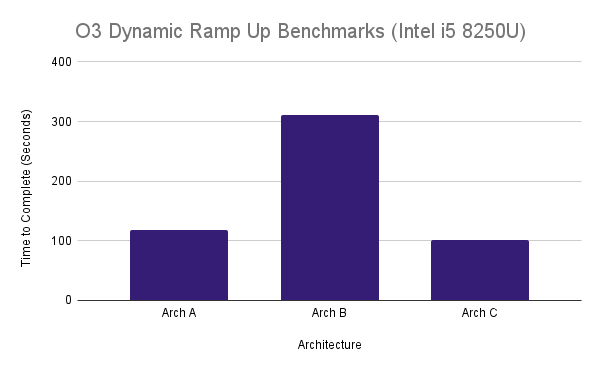
\includegraphics[scale=0.5]{O3 Dynamic Ramp Up Benchmarks (Intel i5 8250U).png}
\label{lapotp_dynamic_ramp_up_tests}
\caption{Dynamic Ramp Up Tests (Intel i5 8250U)}
\end{figure}

\clearpage

\section{Analysis}
\subsection{Architecture A}
\subsubsection{Performance}

\subsubsection{Usability and Maintainability}

\subsection{Architecture B}
\subsubsection{Performance}

\subsubsection{Usability and Maintainability}

\subsection{Architecture C}
\subsubsection{Performance}

\subsubsection{Usability and Maintainability}

\subsection{Architecture D}
\subsubsection{Performance}

\subsubsection{Usability and Maintainability}

\section{Conclusion}

\end{document}
